% !TEX root = ../patchEmbeddings_review.tex

\renewcommand{\thesection}{S\arabic{section}}
\renewcommand{\thetable}{S\arabic{table}}
\renewcommand{\thefigure}{S\arabic{figure}}

\section{Supplementary material}
% \subsection{Averaging overlapping masks}
% In Sec. \ref{sec:aggr_affs}, we introduce a parameter-free algorithm \ref{alg:computing_affinities} to average overlapping masks and extract affinities that can be then used as edge weights of a signed graph with both positive and negative weights. 

% In Fig. \ref{fig:alg_explained}, we show a simplified example of how Algorithm \ref{alg:computing_affinities} computes affinities between a pair of pixels $u$ and $v$.
% In Fig. \ref{fig:mask_cases}, we list the cases in which a \maskname mask can be used or not to predict the affinity between two pixels belonging to the mask.  
% In Fig. \ref{fig:affs_comparison} we compare affinities predicted either by averaging \maskname masks or by directly predicting them as a binary classification output of the model trained with a dense channel-wise S\o rensen-Dice loss.

% Algorithm \ref{alg:computing_affinities} is efficiently implemented on GPU by making use of the \texttt{fold} and \texttt{unfold} functions in PyTorch \cite{NEURIPS2019_9015}. 


\subsection{Graph neighborhood structure and output instance segmentation}
In the first column of Table \ref{tab:neighborhood_structures}, we provide the neighborhood structure of the pixel grid-graph, which is very similar to the one used in related work \cite{wolf2018mutex,lee2017superhuman}.
In Fig. \ref{fig:MWS_segm}, we show the resulting instance segmentation obtained by computing affinities from \maskname masks and then running the Mutex Watershed algorithm on the obtained graph with positive and negative edge weights.

\paragraph{Removing small segments} -- After running the Mutex Watershed, we use a simple post-processing step to delete small segments on the boundaries, most of which are given by single-voxel clusters. On the neuron segmentation predictions, we deleted all regions with less than 200 voxels and used a seeded watershed algorithm to expand the bigger segments.


\subsection{Details on the model architecture}\label{sec:arch_details_suppl}
Fig. \ref{fig:model_architecture} shows the details on the 3D-UNet architecture and Table \ref{tab:neighborhood_structures} lists the sparse neighborhood structures predicted by the \emph{\sparseBr branches}. Only the outputs at the highest resolution (given by branches SNB$_1$, ENB$_1$ and ENB$_2$) are used to compute edge weights in the pixel grid-graph. A visualization of the predicted single-instance mask latent spaces is given in Fig. \ref{fig:PCA_embeddings}.
% - Cite architecture figure Fig: we use three type of nets, we only use highest res predictions for computing affinities of the graph

The input volume has shape $272 \times 272\times12$ which is equivalent to a volume of $544\times 544\times 12$ voxels in the original resolution $4\times 4\times 40$ nm$^3$. Before to apply the loss, we crop the predictions to a shape $224\times 224\times 9$ in order to avoid border artifacts\footnote{Instead of cropping directly the final predictions, we perform several crops in the decoder part of the UNet model (see Upsample + Crop connections in Fig. \ref{fig:model_architecture}) in order to optimize GPU-memory usage.}.
The final model trained on all available ground truth labels is trained with a slightly larger input volume of $288\times 288\times 14$.



% \begin{itemize}
% \item residual blocks with group normalization layers and skip-connections involving sum of feature maps from 
% \item The input volume has shape $272 \times 272\times12$ which is equivalent to a volume of $544\times 544\times 12$ voxels in the original resolution $4\times 4\times 40$ nm$^3$. Before to apply the loss, we crop the predictions to a shape $224\times 224\times 9$ in order to avoid border artifacts. 
% The final model trained on all available ground truth labels is trained with a slightly larger input volume of $288\times 288\times 14$ and we provide even more input to the cheaper glia-predictor-model: $352\times 352\times 15$ voxels. 
% \item Explicitly say what is the size of the coarsest predicted mask in the original res, which should be $112 \times 112 \times 5$ voxels at res...
% \item which outputs do we use for the averaging stuff? Only the high-res ones
% \item Crops in the decoder part
% \item In the supplementary material, we provide all the architecture details: crops in the decoder of the UNet
% \item we predict two types of \maskname masks at the highest level of the hierarchy
% \item Post-processing (remove small segments)
% \item we only use the outputs at the highest resolution for predicting affinities!
% \item we either use all, only SNB or only ENB
% \end{itemize}






% \textbf{Glia classifier} -- As a final post-processing step, we merge neighboring instances that have been classified as \emph{glia segments} (putative astrocyte). This is a common procedure in neuron segmentation \TODO{CIT}\cite{lee2019learning}, since glia segments are substantially different from the other neurons and are usually considered separately in the final reconstructed diagram of neural circuit connectivity. Glia segments usually present a main body with a lot of very thin glial processes




% \begin{figure}[t]
% \begin{subfigure}[t]{0.47\linewidth}
% \centering
% 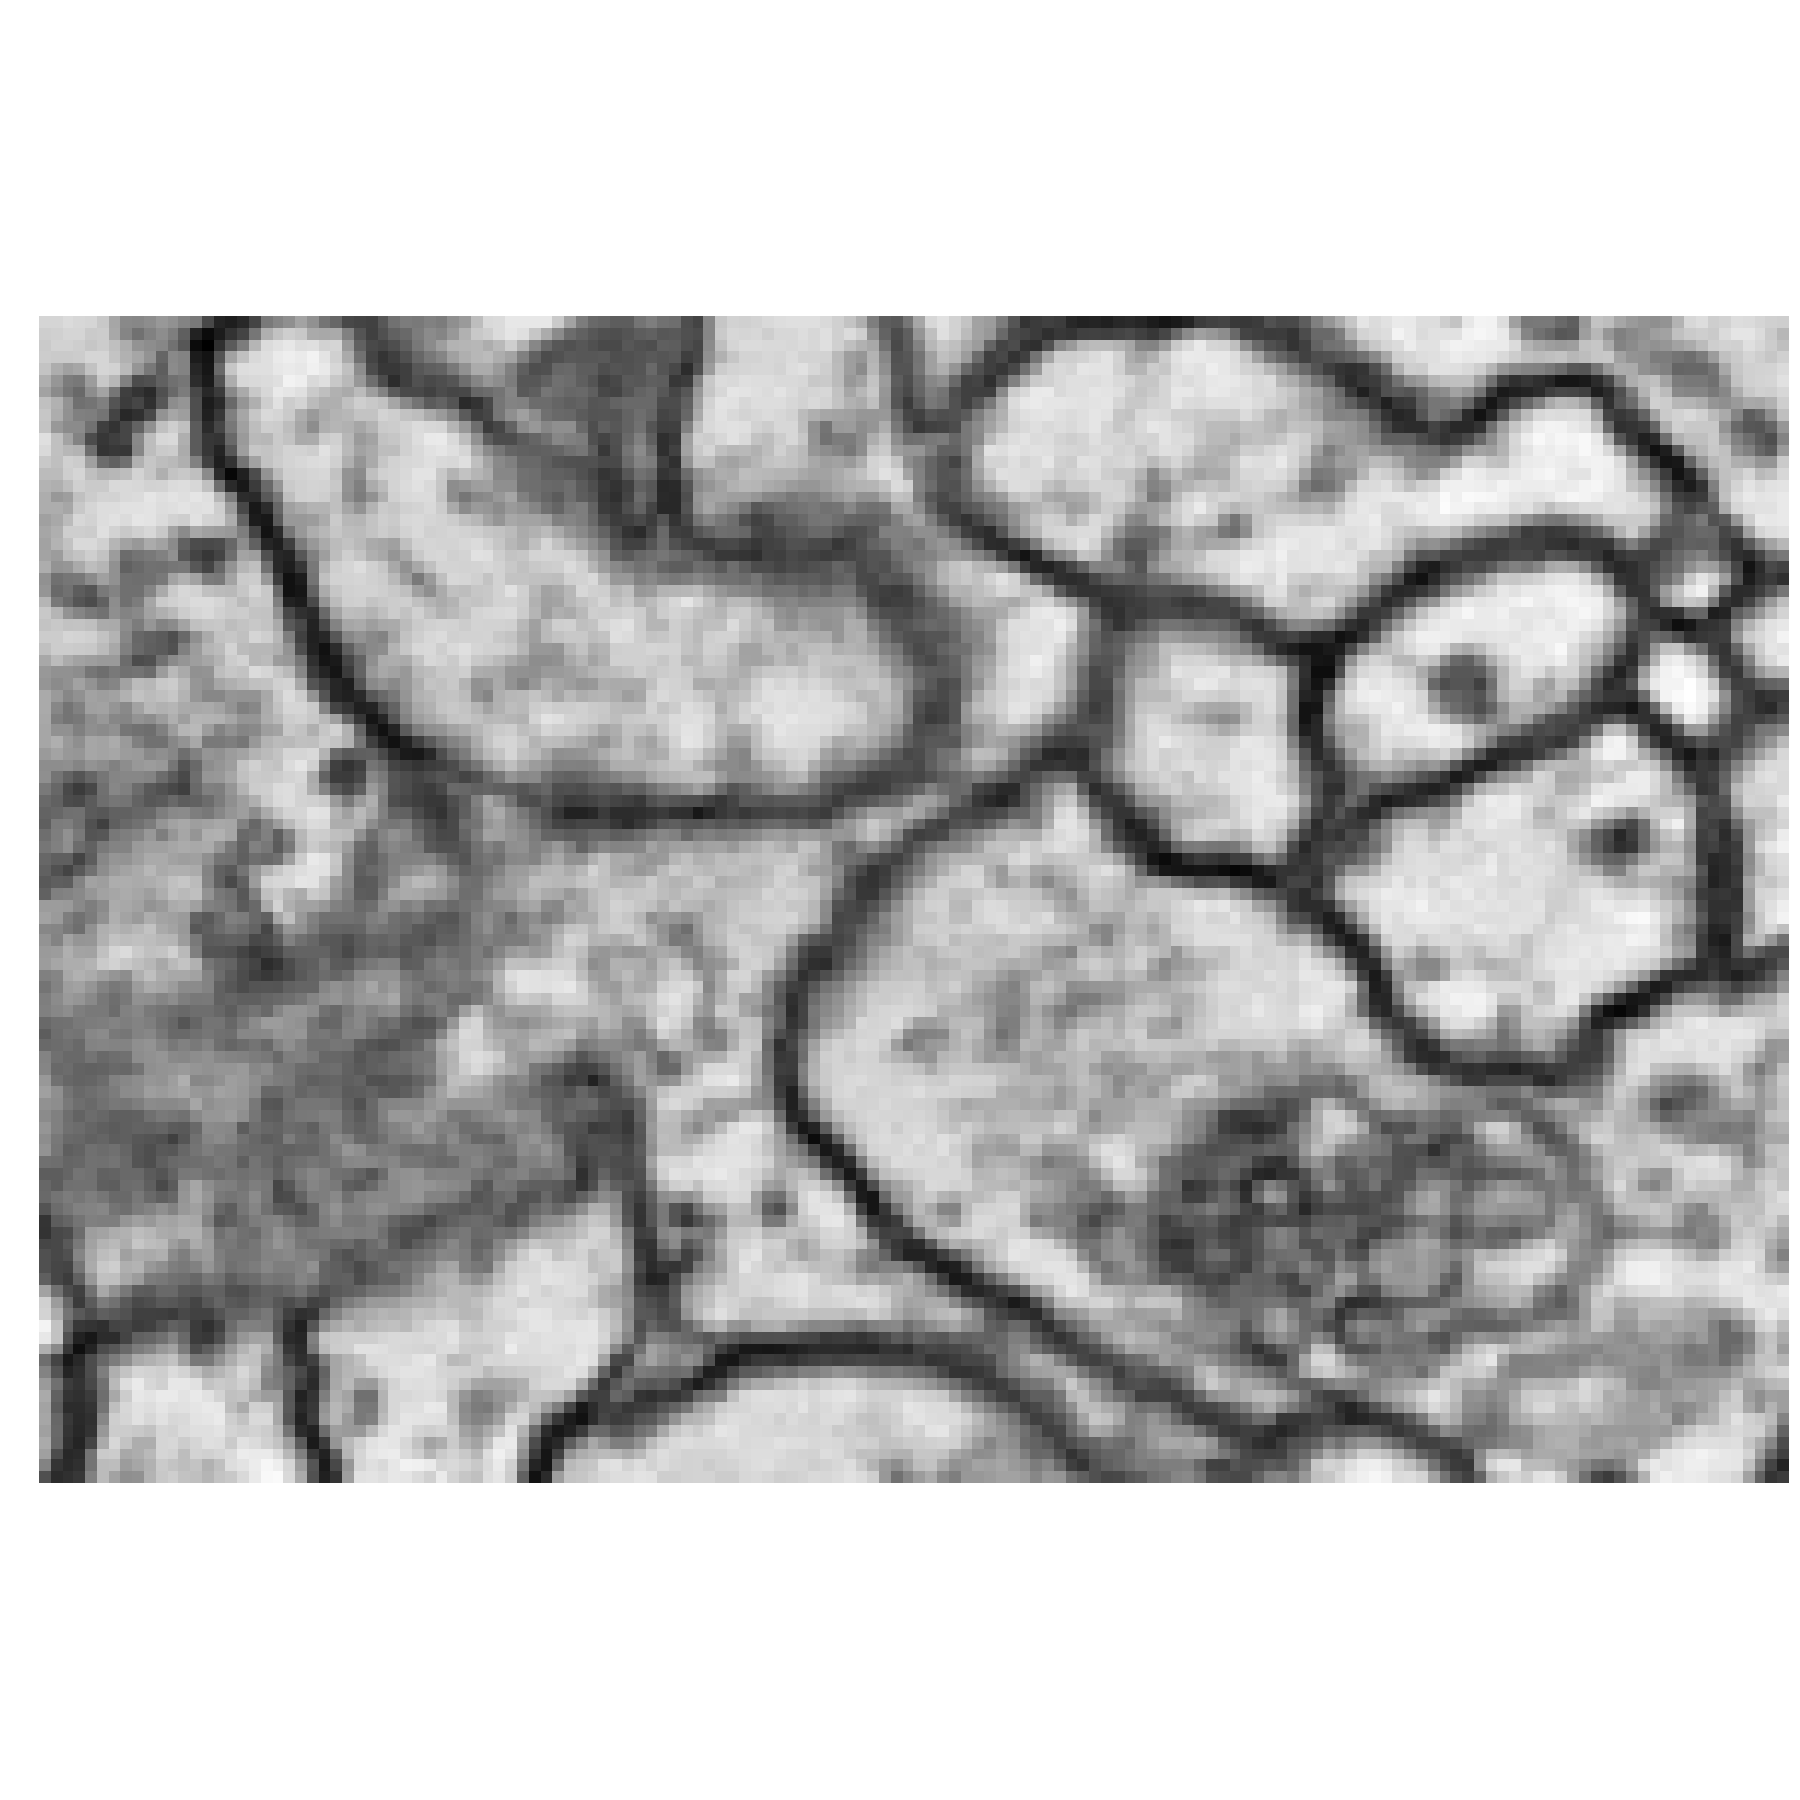
\includegraphics[width=0.65\linewidth,trim=1.50in 1.4in 1.4in 1.50in,clip]{./figs/affs_compare/raw_mod.pdf} % 
% \caption{\centering Raw image}
% \end{subfigure}\hfill
% \begin{subfigure}[t]{0.47\textwidth}
% \centering
% 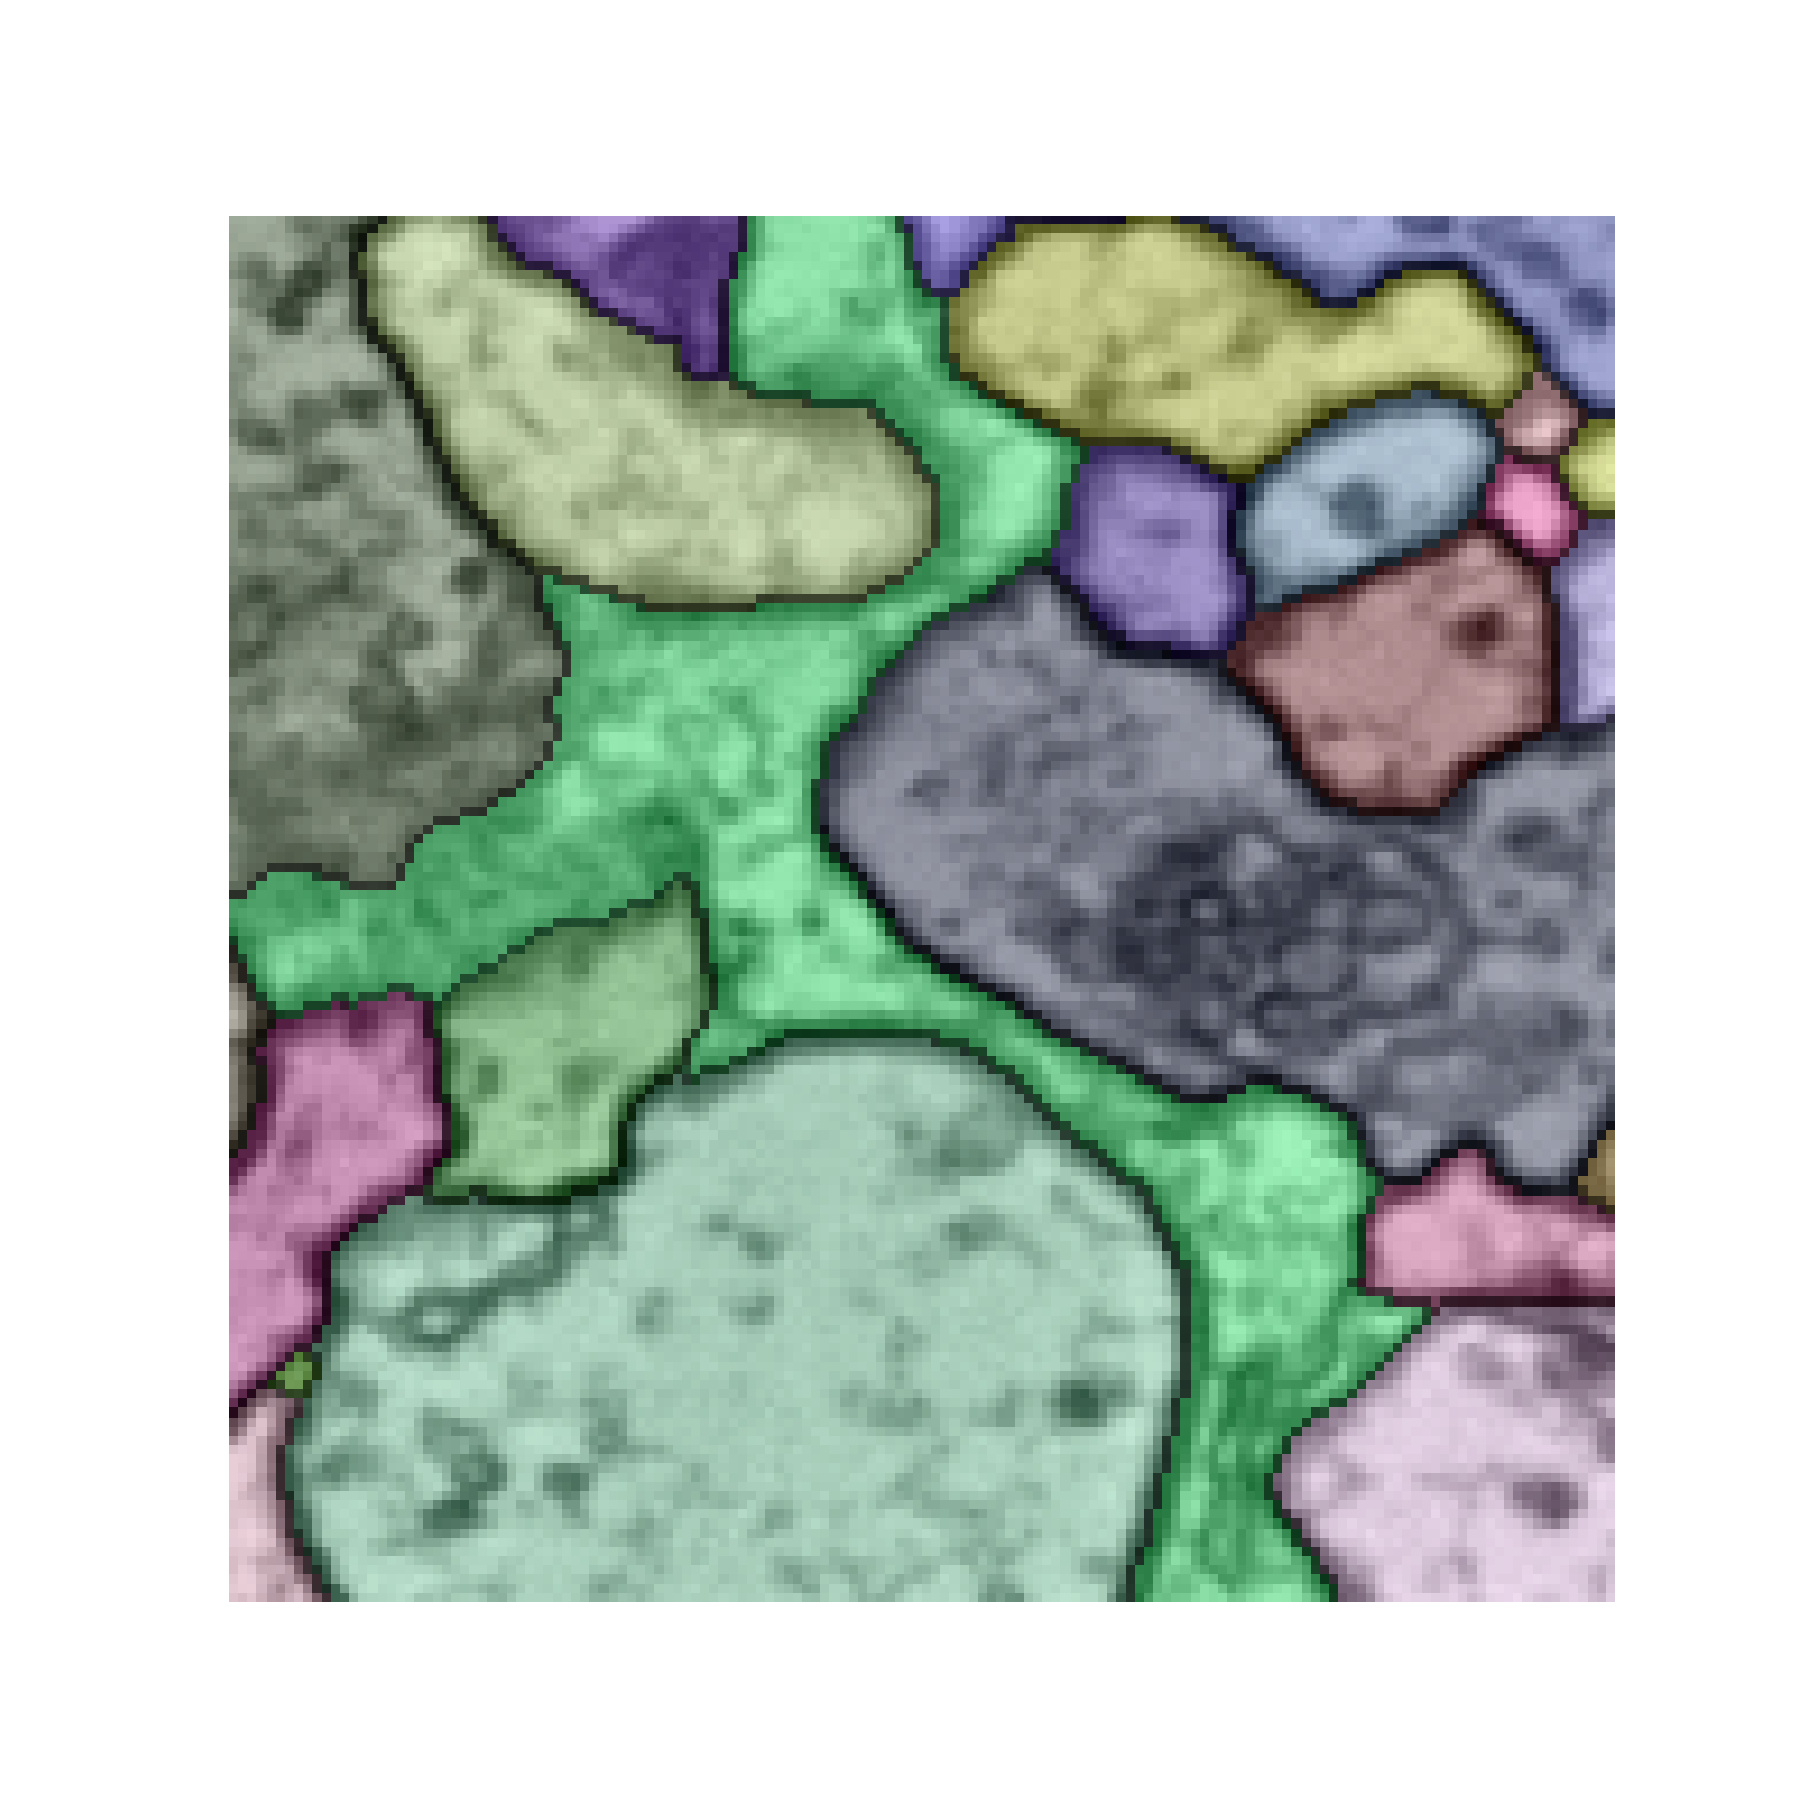
\includegraphics[width=0.65\linewidth,trim=1.50in 1.4in 1.4in 1.50in,clip]{./figs/affs_compare/GT.pdf} % ,trim=0.25in 0.25in 0.65in 0.36in,clip
% \caption{\centering Ground truth segmentation overlaid with the raw image}
% \end{subfigure}\vspace{2em}\\
% \begin{subfigure}[t]{0.47\linewidth}
% \centering
% 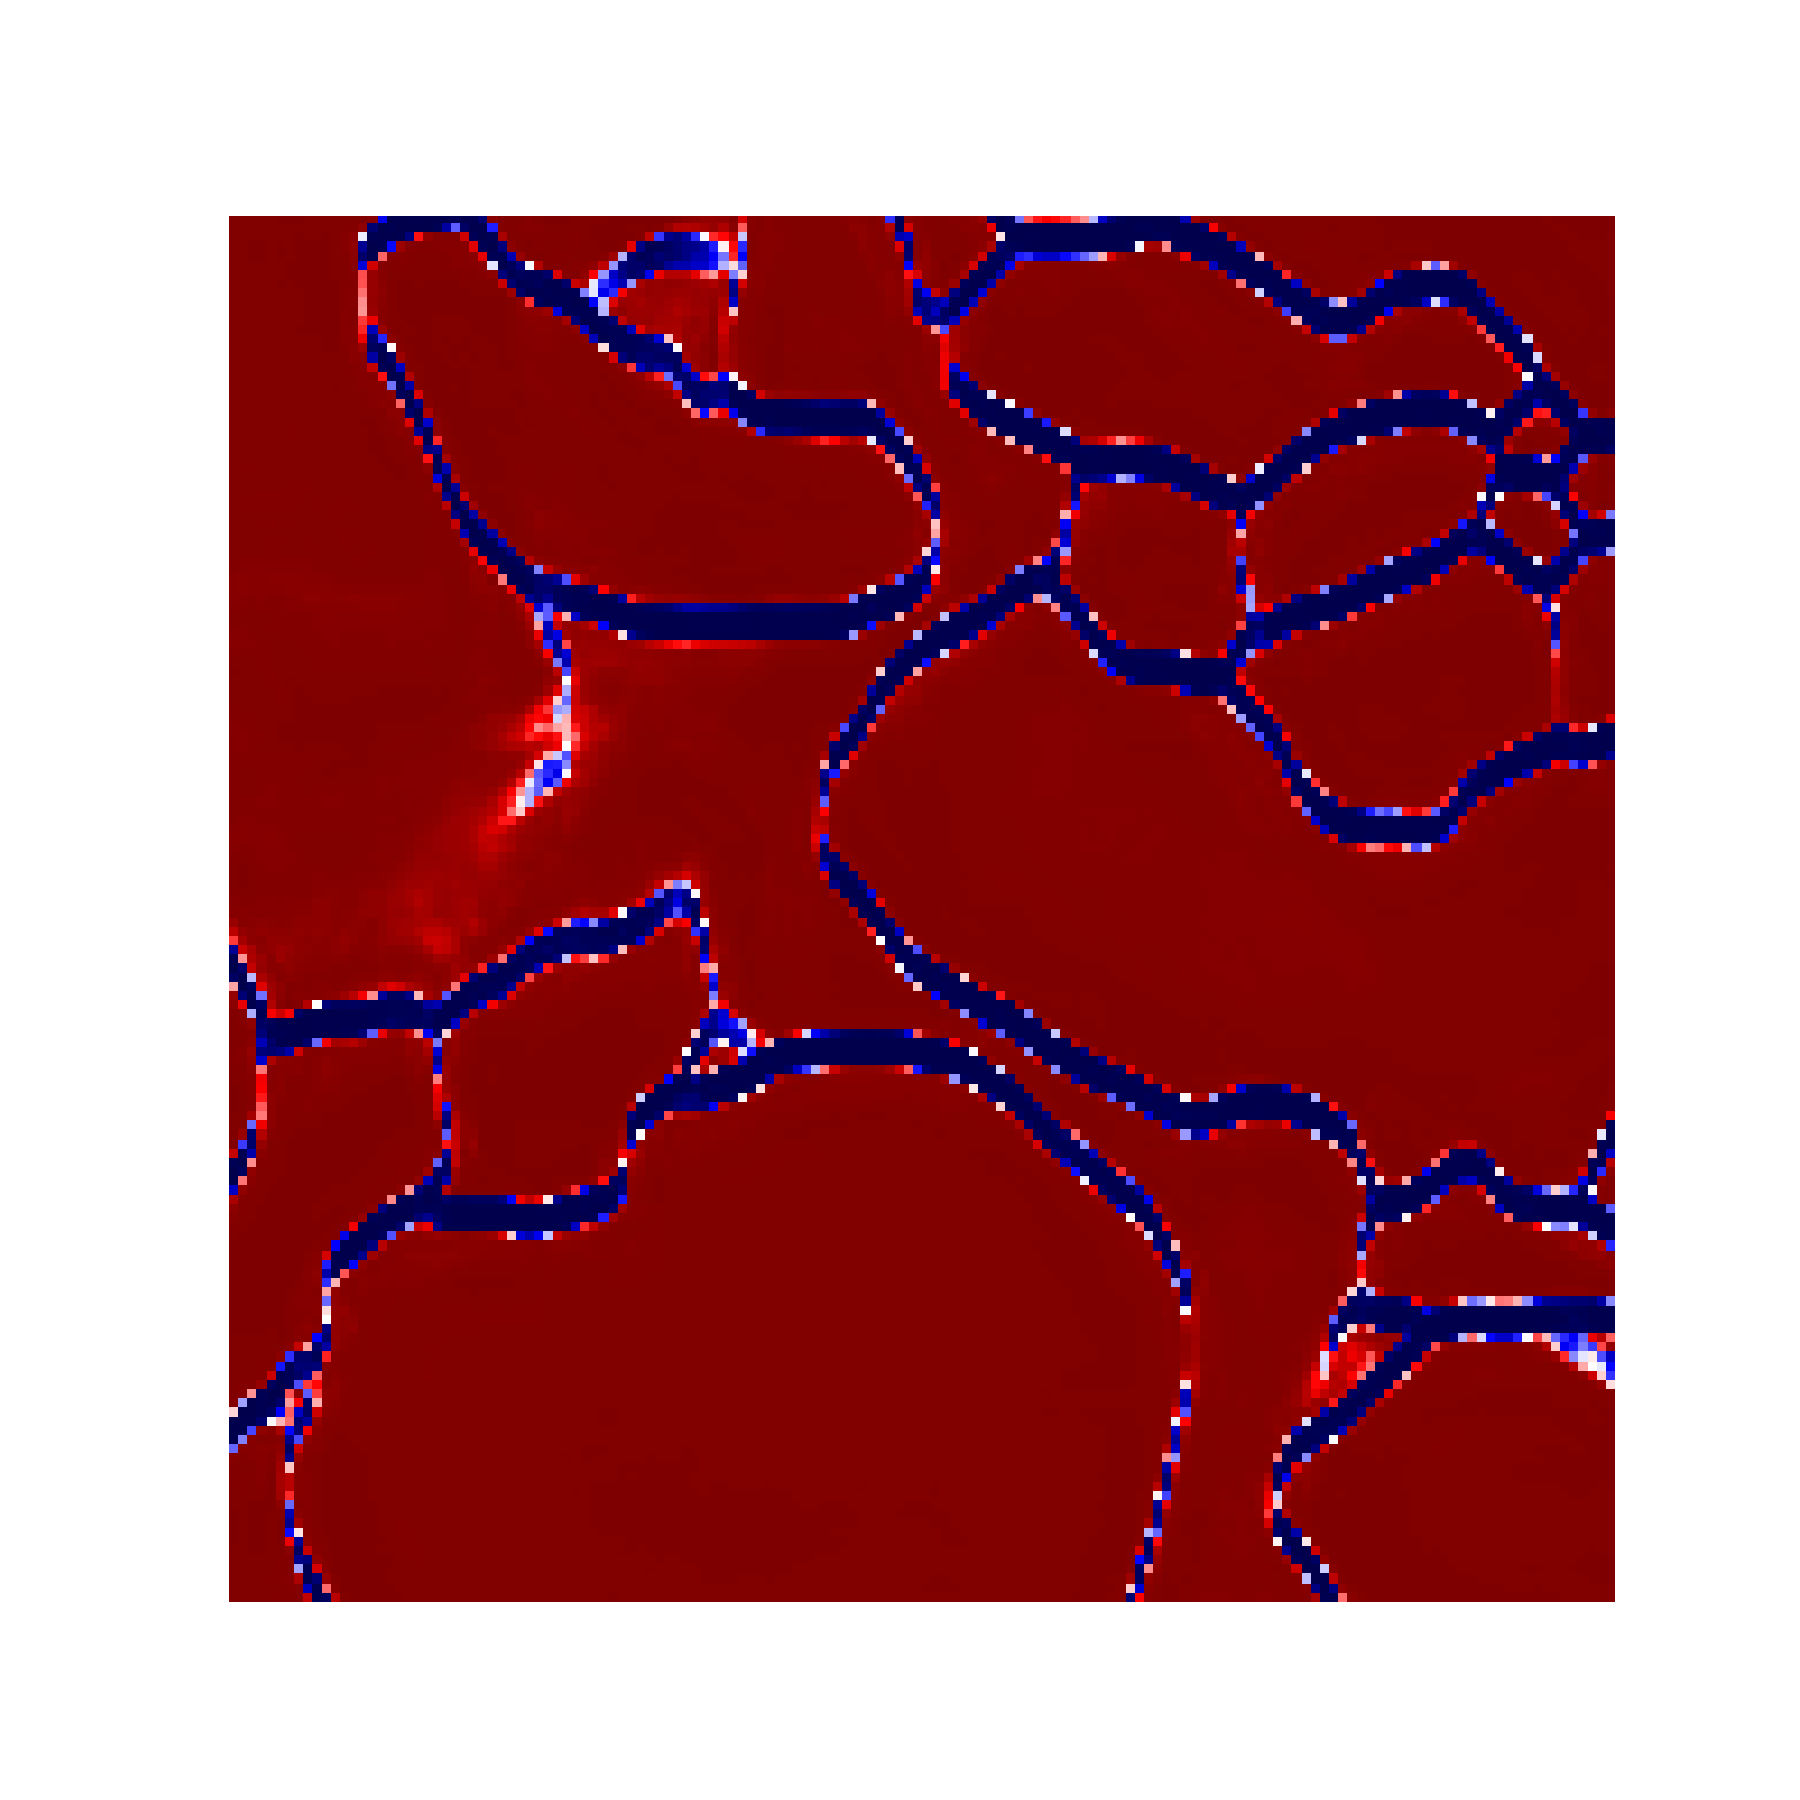
\includegraphics[width=0.65\linewidth,trim=1.50in 1.4in 1.4in 1.50in,clip]{./figs/affs_compare/affs1.pdf} % ,trim=0.25in 0.25in 0.65in 0.36in,clip
% \caption{\centering Affinities trained with S\o rensen-Dice loss (along vertical direction)}
% \end{subfigure}\hfill
% \begin{subfigure}[t]{0.47\textwidth}
% \centering
% 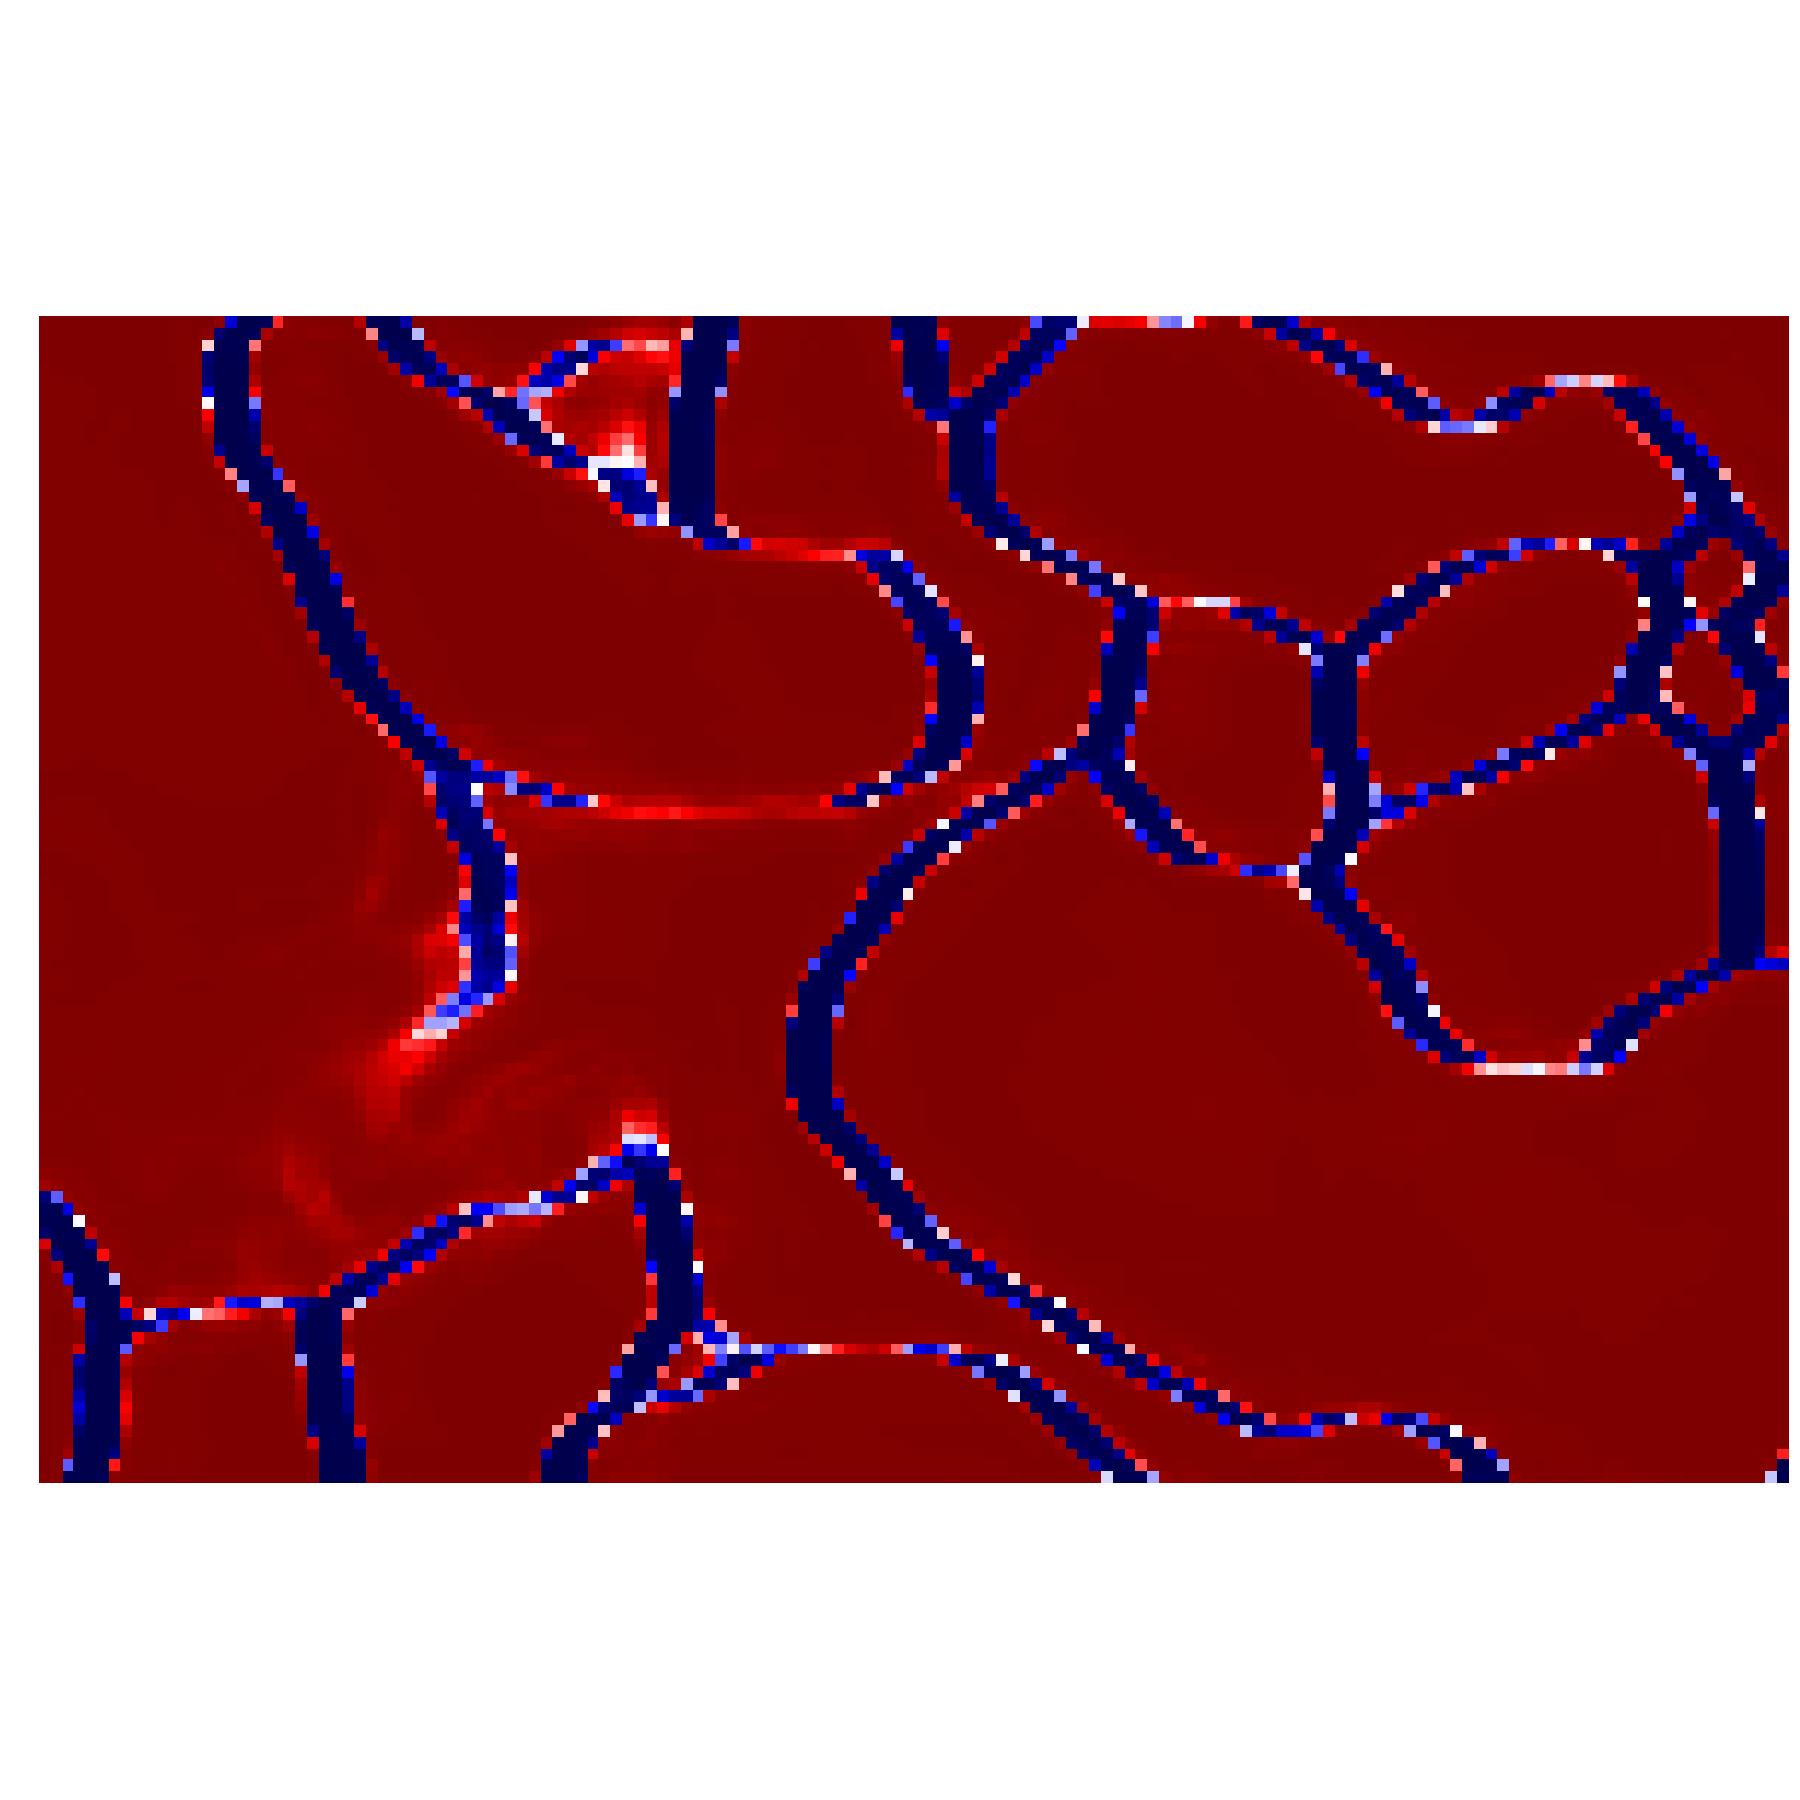
\includegraphics[width=0.65\linewidth,trim=1.50in 1.4in 1.4in 1.50in,clip]{./figs/affs_compare/affs2.pdf} % ,trim=0.25in 0.25in 0.65in 0.36in,clip
% \caption{\centering Affinities trained with S\o rensen-Dice loss (along horizontal direction)}
% \end{subfigure}\vspace{2em}\\
% \begin{subfigure}[t]{0.47\linewidth}
% \centering
% 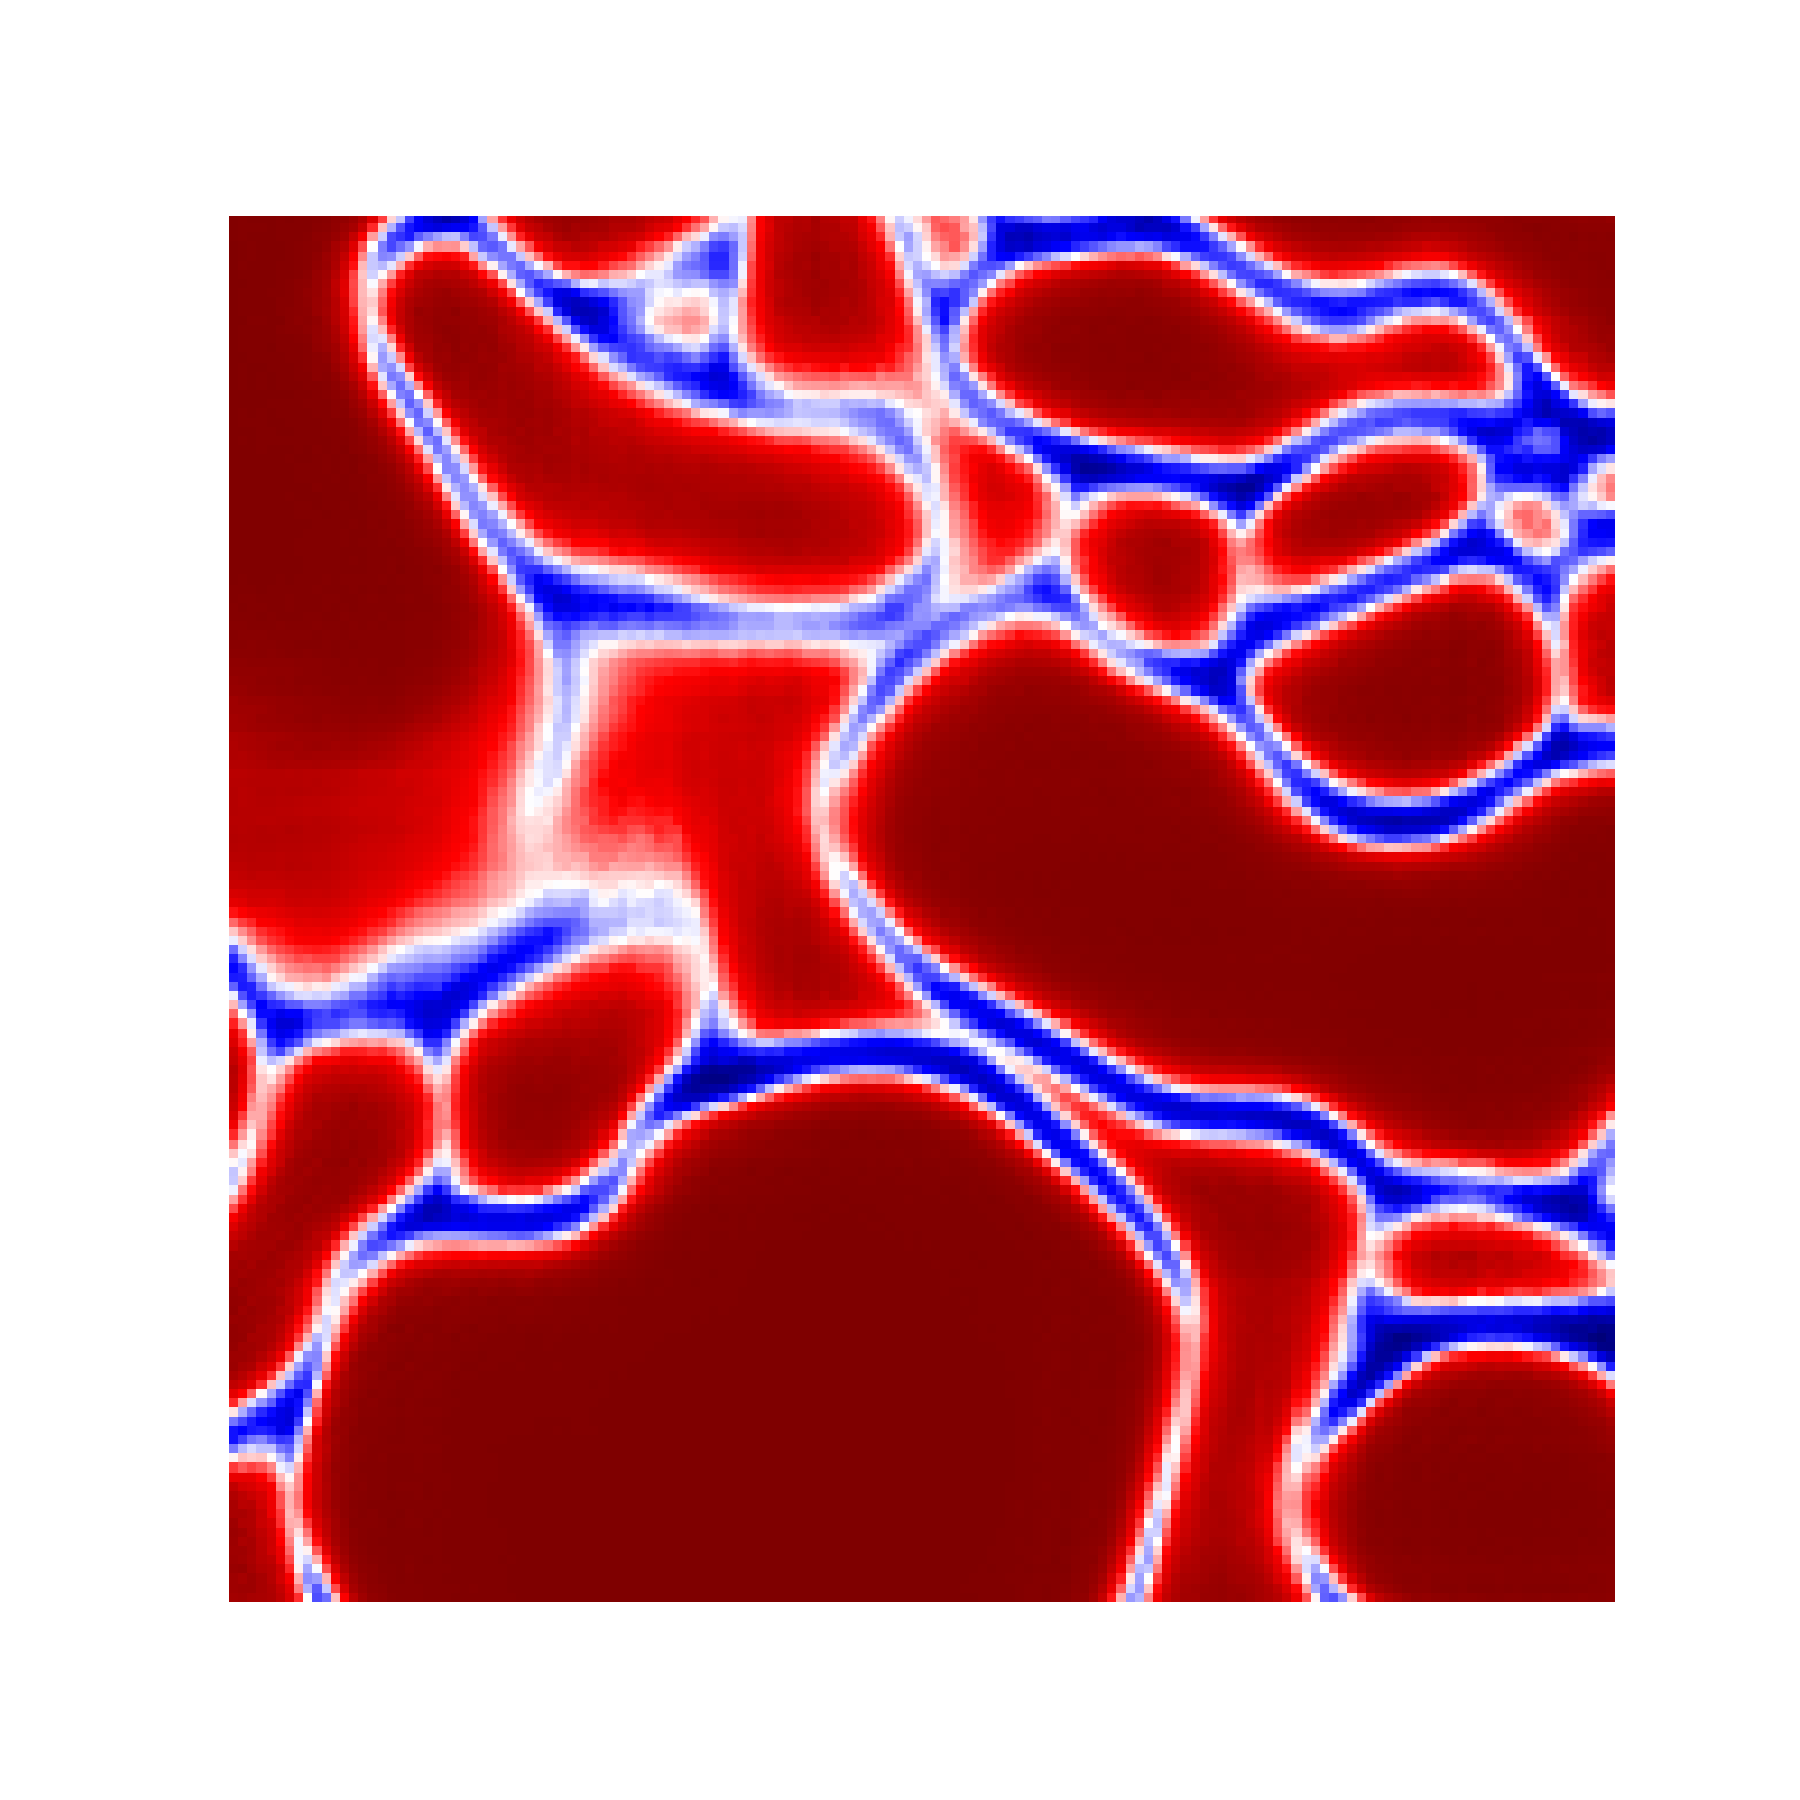
\includegraphics[width=0.65\linewidth,trim=1.50in 1.4in 1.4in 1.50in,clip]{./figs/affs_compare/affs3.pdf} % ,trim=0.25in 0.25in 0.65in 0.36in,clip
% \caption{\centering Affinities from averaging overlapping masks (along vertical direction)}
% \end{subfigure}\hfill
% \begin{subfigure}[t]{0.47\textwidth}
% \centering
% 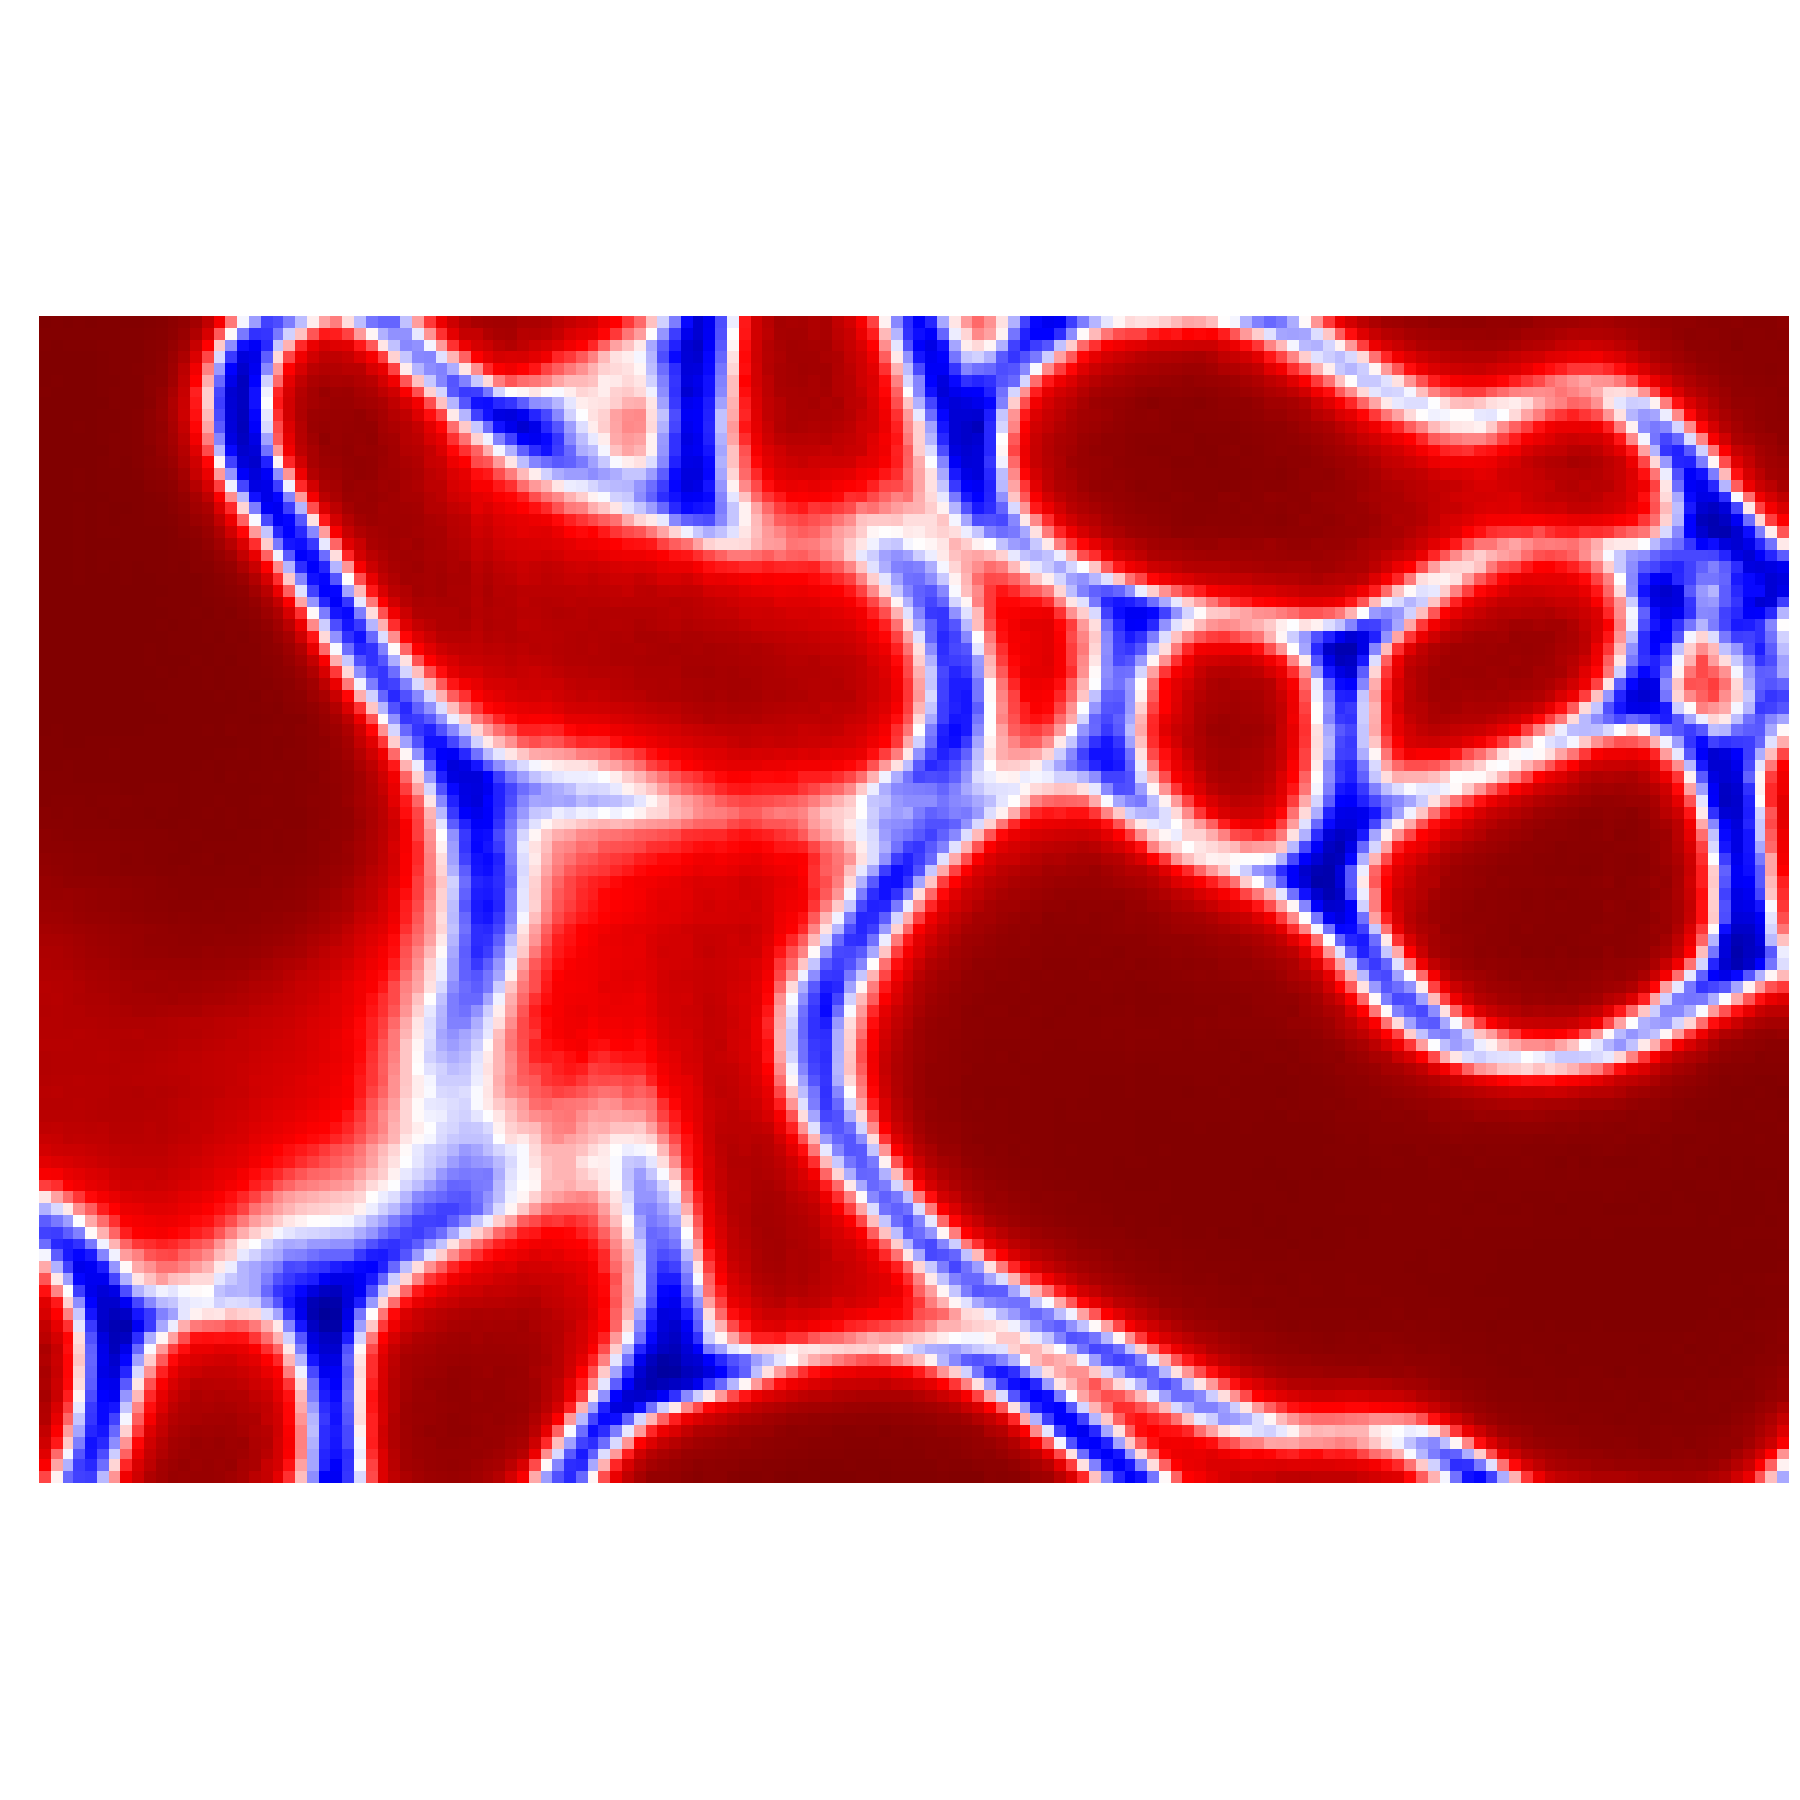
\includegraphics[width=0.65\linewidth,trim=1.50in 1.4in 1.4in 1.50in,clip]{./figs/affs_compare/affs4.pdf} % ,trim=0.25in 0.25in 0.65in 0.36in,clip
% \caption{\centering Affinities from averaging overlapping masks (along horizontal direction)}
% \end{subfigure}
% \caption{Comparison between different ways of predicting affinities and their robustness to noise. \textbf{(a-b)} Raw data and  associated ground-truth labels. \textbf{(c-d)} Affinities predicted by the \emph{sparse-neighborhood branch}, which is trained with a dense channel-wise S\o rensen-Dice loss (high affinities are represented in red, low ones in blue). \textbf{(e-f)} Affinities computed by averaging overlapping masks (AffAggr). We note how averaged affinities are smoother and present a more consistent boundary evidence in the noisy region highlighted by the red circle. In these plots we show two types of affinities representing neighborhood relations along the horizontal (-4, 0, 0) and vertical (0, -4, 0) directions.}\label{fig:affs_comparison}
% \end{figure}

\begin{figure}[t]
\centering
        % \includegraphics[width=0.4\textwidth,trim=0.25in 0.25in 0.68in 0.36in,clip]{./figs/SSBM_experiments.pdf} % 0.45
        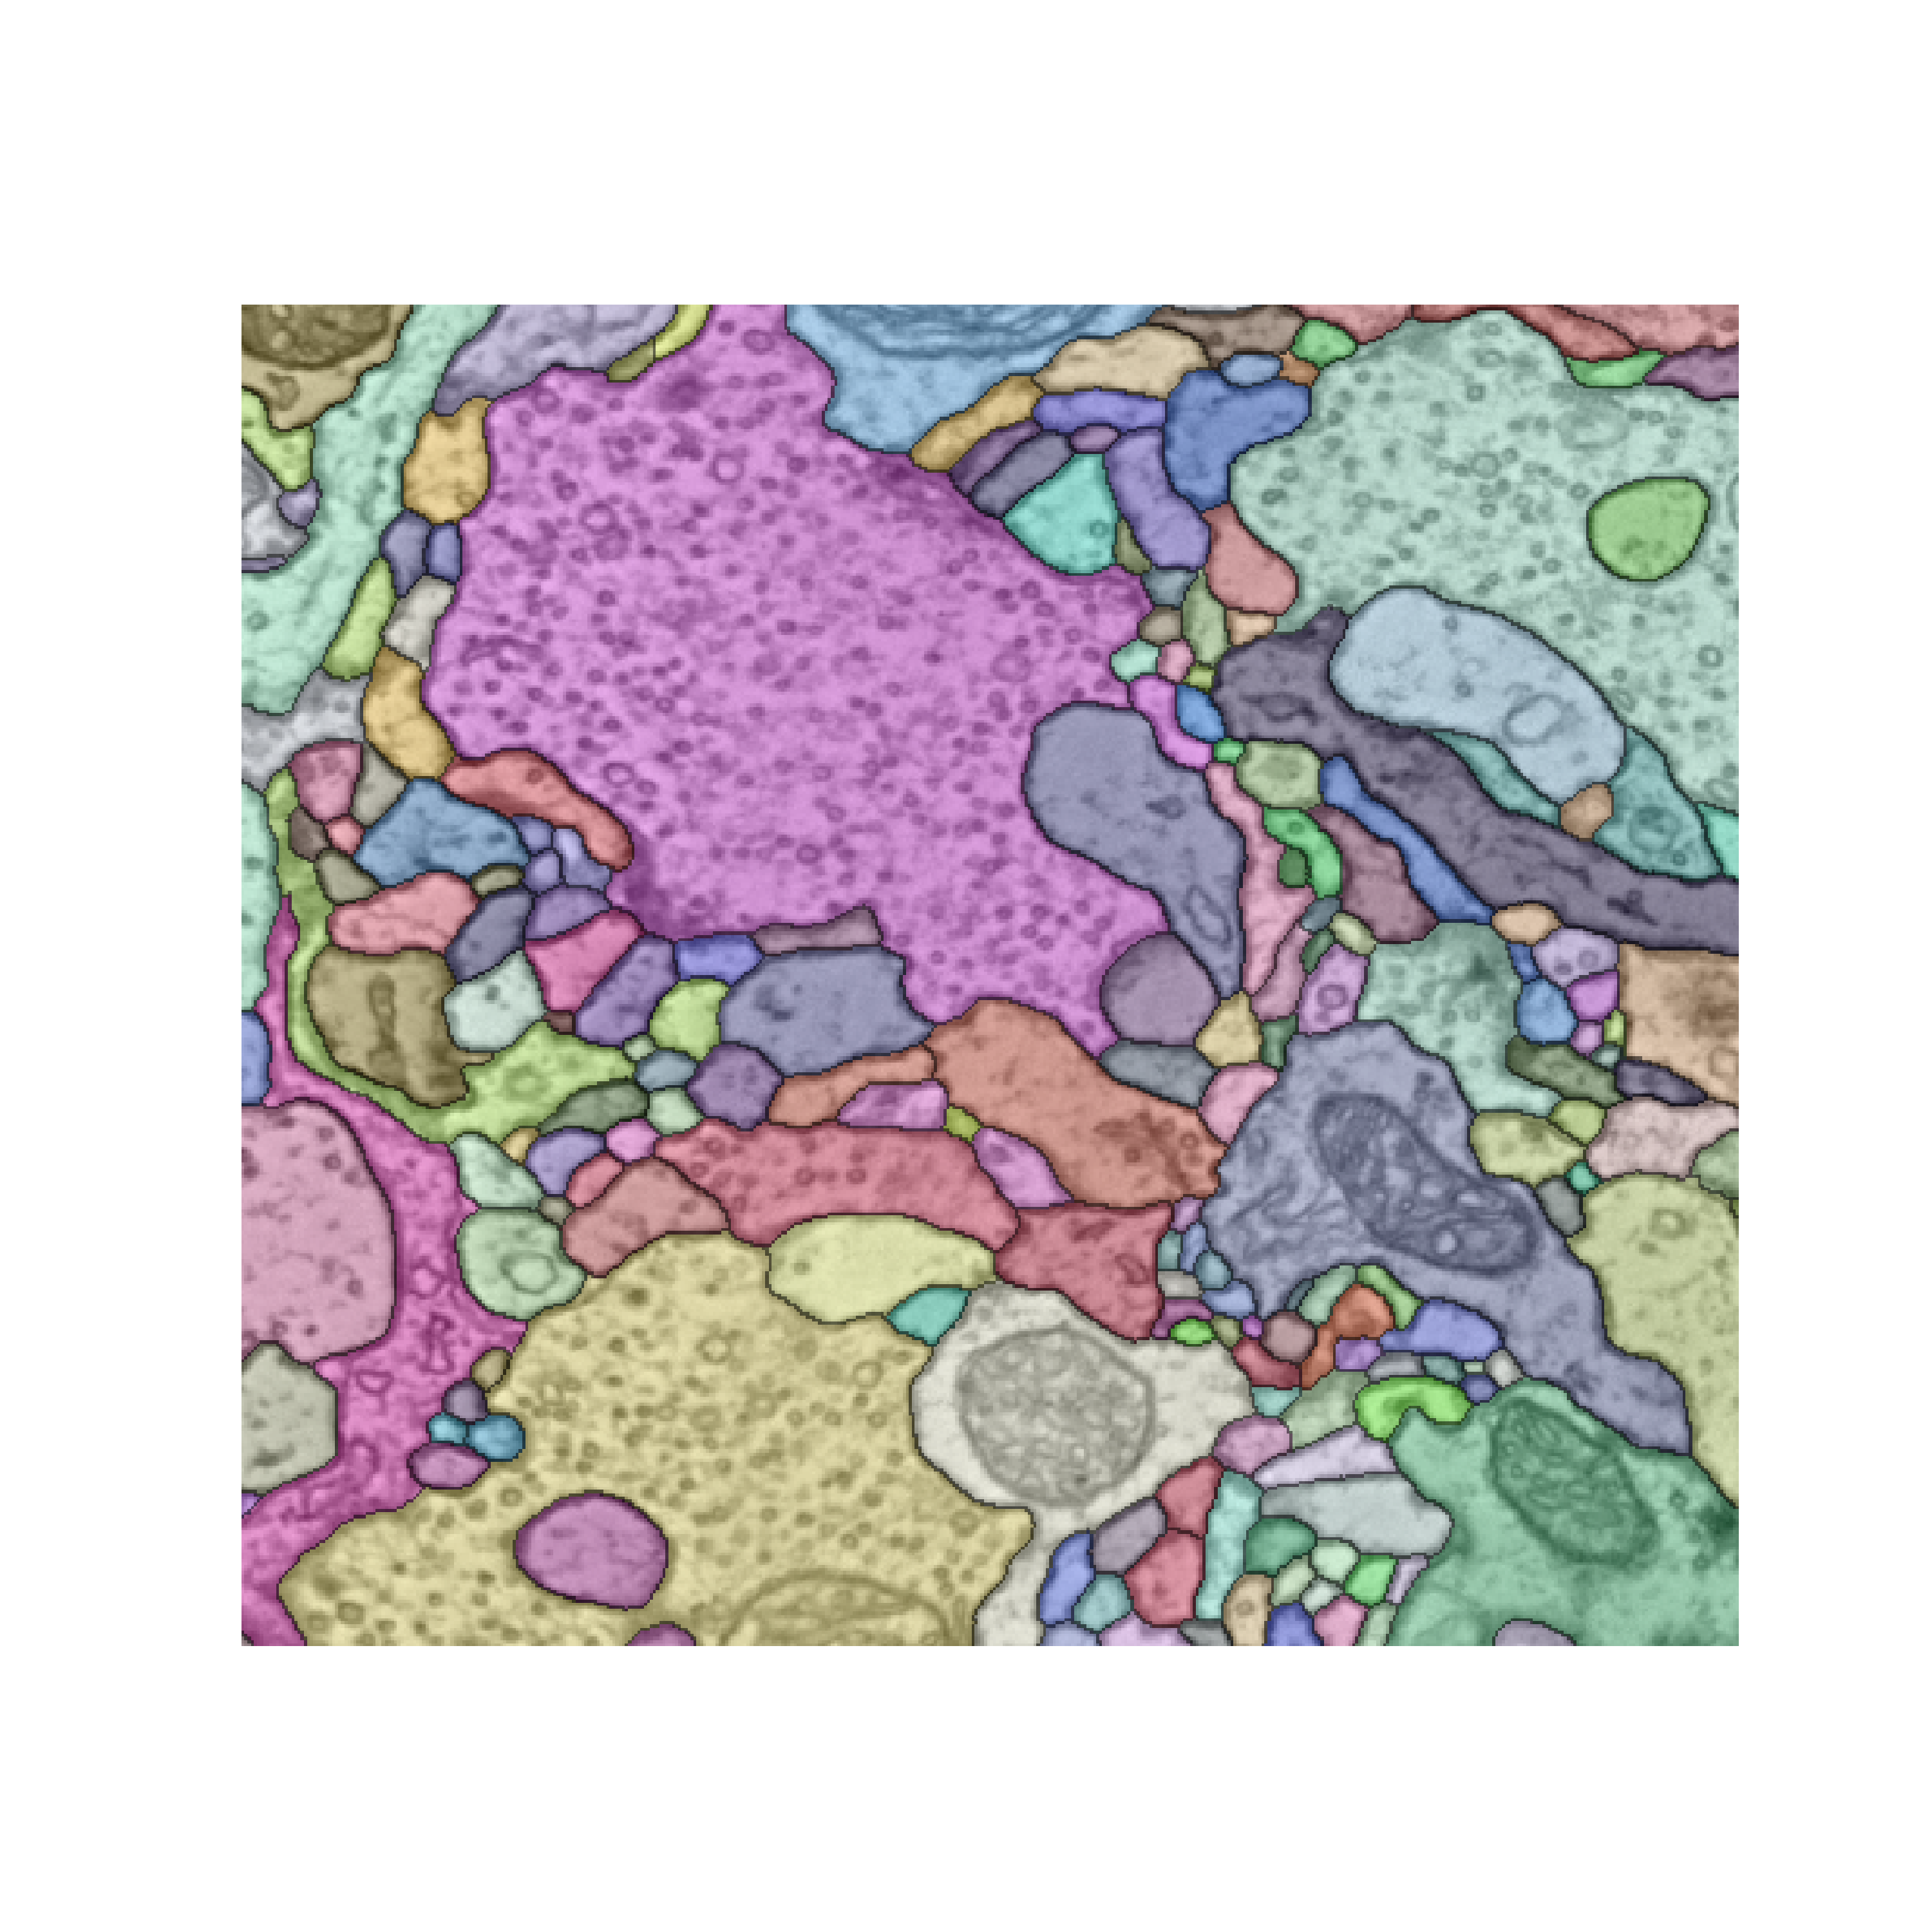
\includegraphics[width=\textwidth,trim=1.80in 1.4in 1.8in 1.50in,clip]{./figs/MWS_segm.pdf} % 0.45
        \caption{Raw data from the validation set overlaid with the final instance segmentation obtained with our method: affinities are computed by averaging overlapping masks (MaskAggr); the final segmentation is achieved by running the Mutex Watershed algorithm on the obtained graph with positive and negative edge weights. Note that the data is 3D, hence the same color could be assigned to parts of segments that appear disconnected in 2D.}
    \label{fig:MWS_segm}
\end{figure}




\begin{figure}[t]
\centering
        % \includegraphics[width=0.4\textwidth,trim=0.25in 0.25in 0.68in 0.36in,clip]{./figs/SSBM_experiments.pdf} % 0.45
        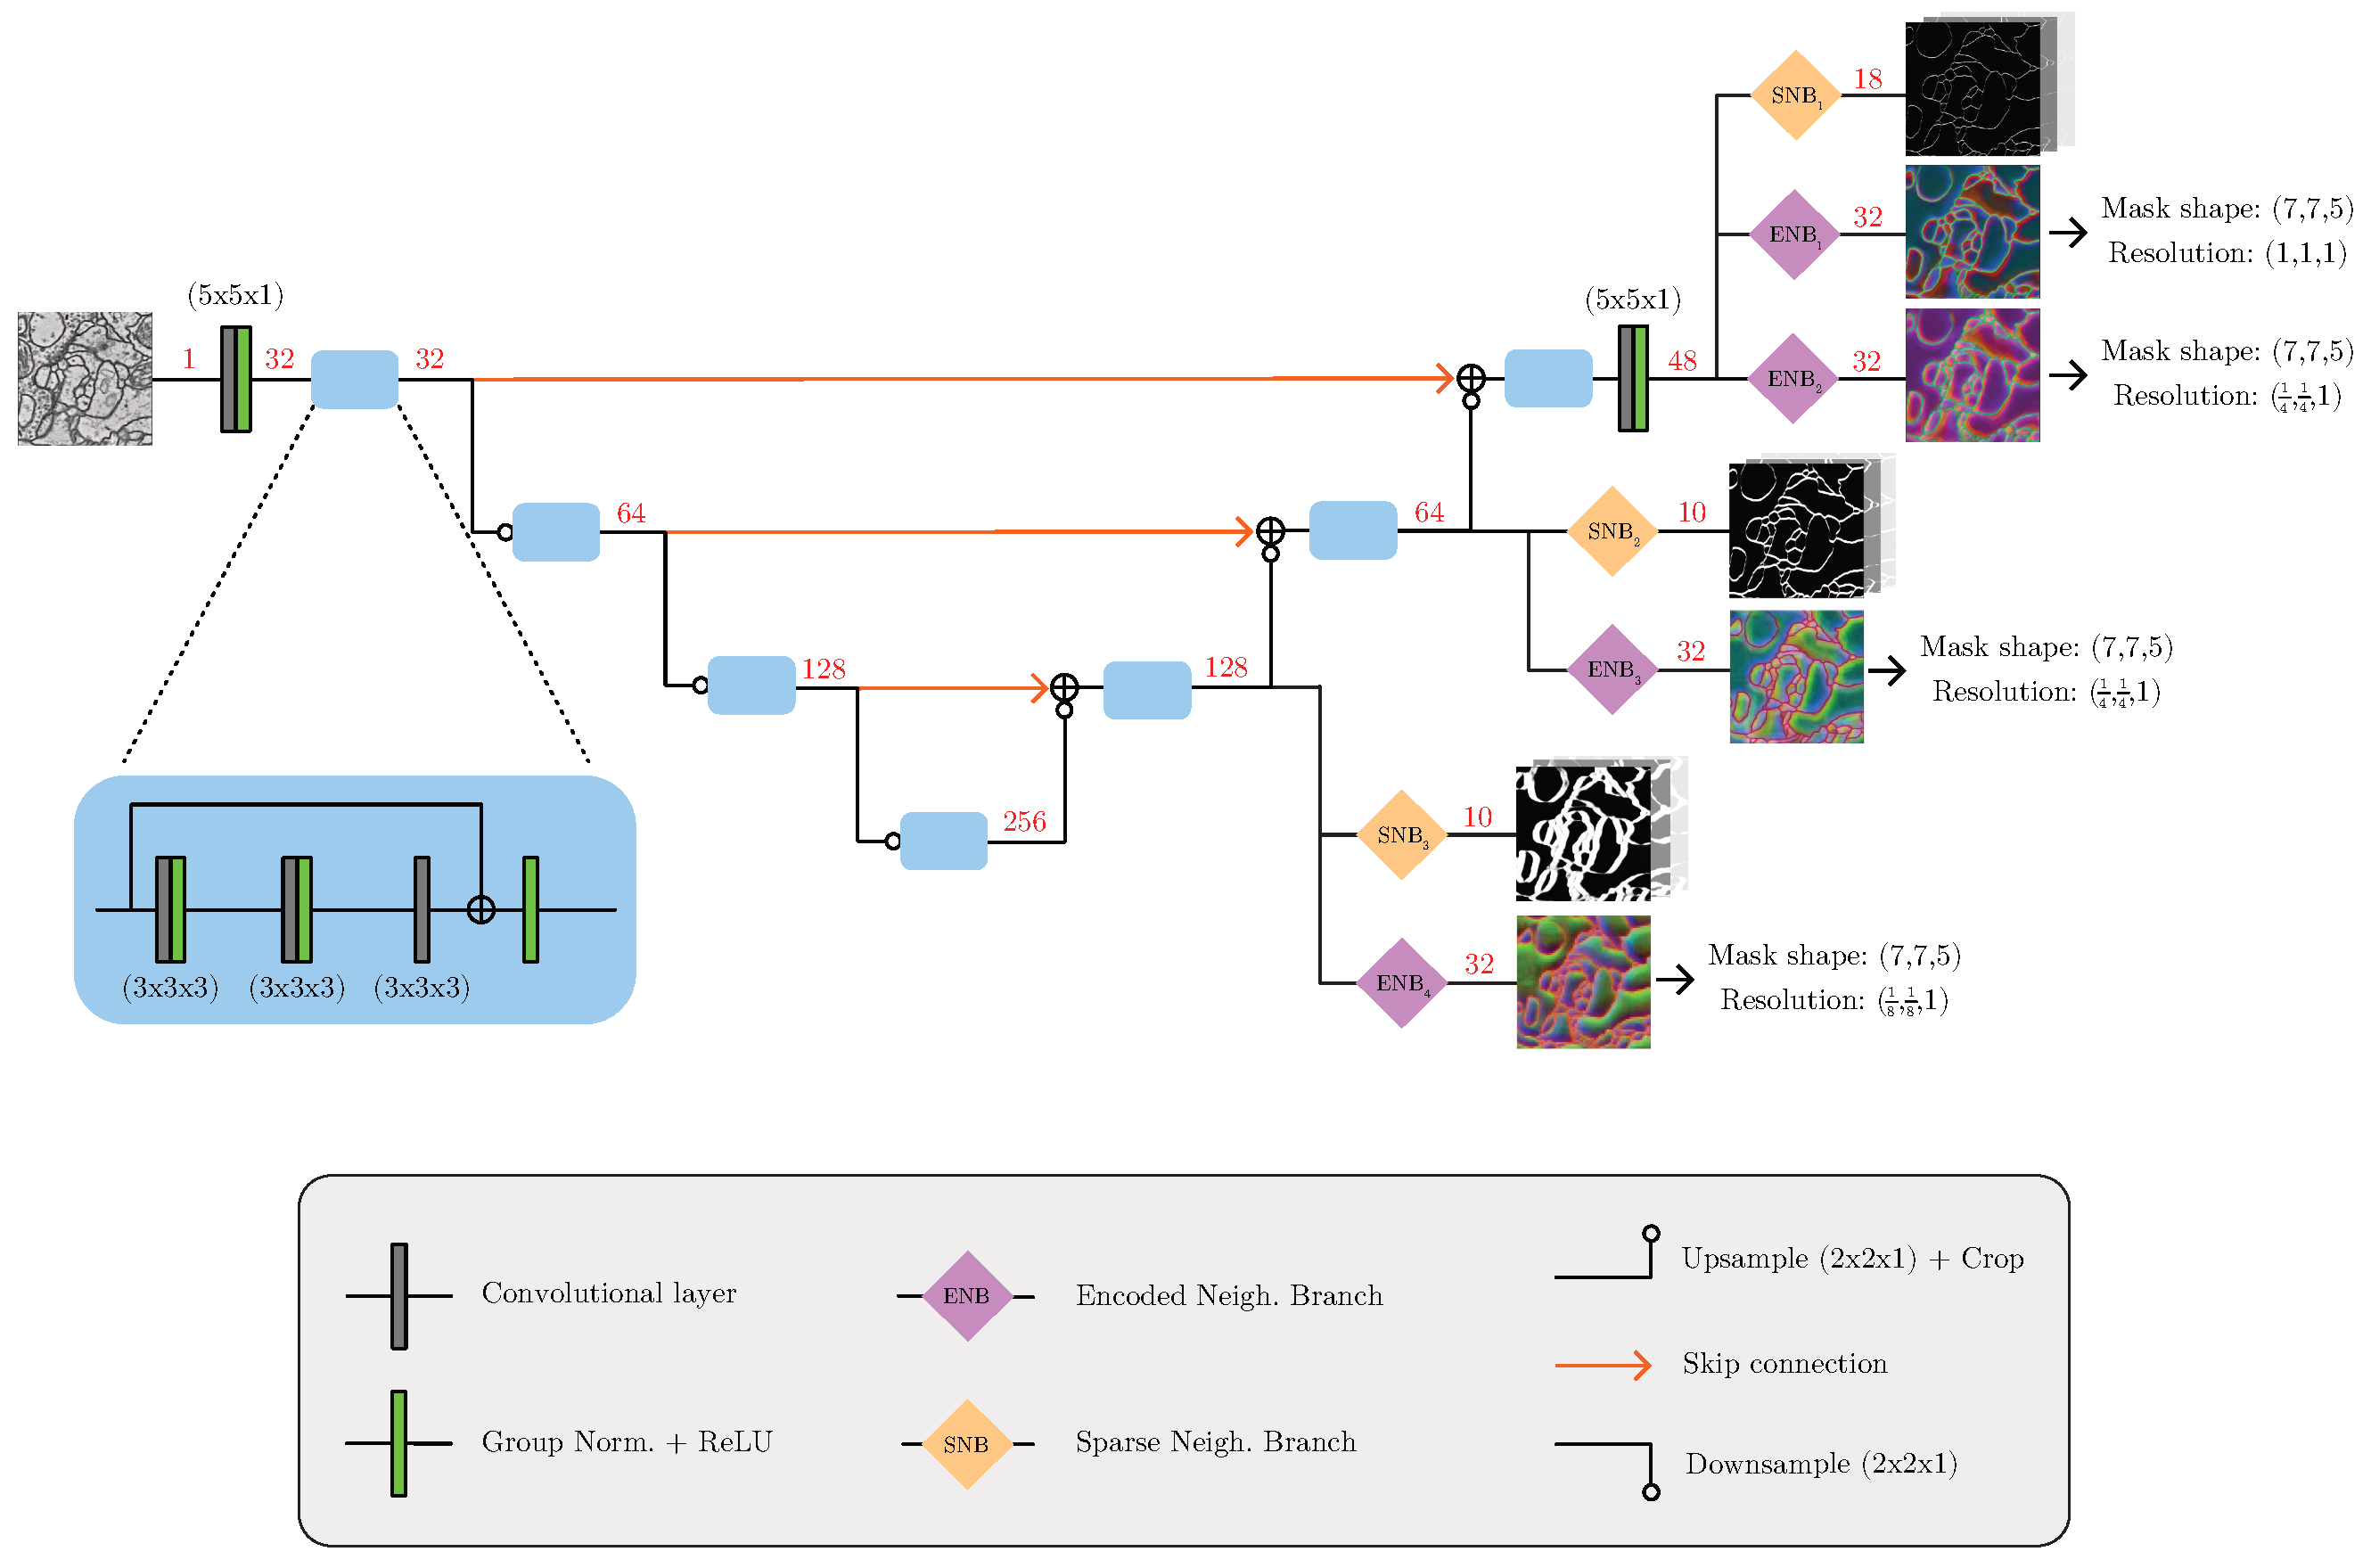
\includegraphics[width=\textwidth]{./figs/UNet_architecture.pdf} % 0.45
        \vspace{1em}
        \caption{\textbf{The architecture of the model}, which is strongly inspired by the 3D-UNet models proposed in \cite{lee2017superhuman,funke2018large}. 
        Red numbers indicate the number of used feature maps.
        As we explain in Sec. \ref{sec:models_details}, in this work we consider three models: i) a baseline model based on the three \emph{\sparseBr branches} SNB$_{i=1,2,3}$, shown in the figure; ii) another model based on the four \emph{\encBr branches} ENB$_{i=1,2,3,4}$; iii) and, finally, a combined model trained with all seven branches shown in the Figure.
        Even though the input of the model is a 3D volume, here, for simplicity, we show an example of 2D input image taken from the stack. As output of the \emph{\sparseBr branches} SNB$_{i=1,2,3}$, we show few channels representing some of the predicted affinities (see Table \ref{tab:neighborhood_structures} for details on the sparse neighborhood structures predicted by each branch SNB$_{i=1,2,3}$). We also show the first three principal components of the encoded masks predicted by the \emph{\encBr branches} ENB$_{i=1,2,3,4}$. All branches ENB$_{i=1,2,3,4}$ predict \maskname masks of the same window size $7 \times 7 \times 5$, but at different resolutions.}
    \label{fig:model_architecture}
\end{figure}

\begin{figure}[t]
\centering
        % \includegraphics[width=0.4\textwidth,trim=0.25in 0.25in 0.68in 0.36in,clip]{./figs/SSBM_experiments.pdf} % 0.45
        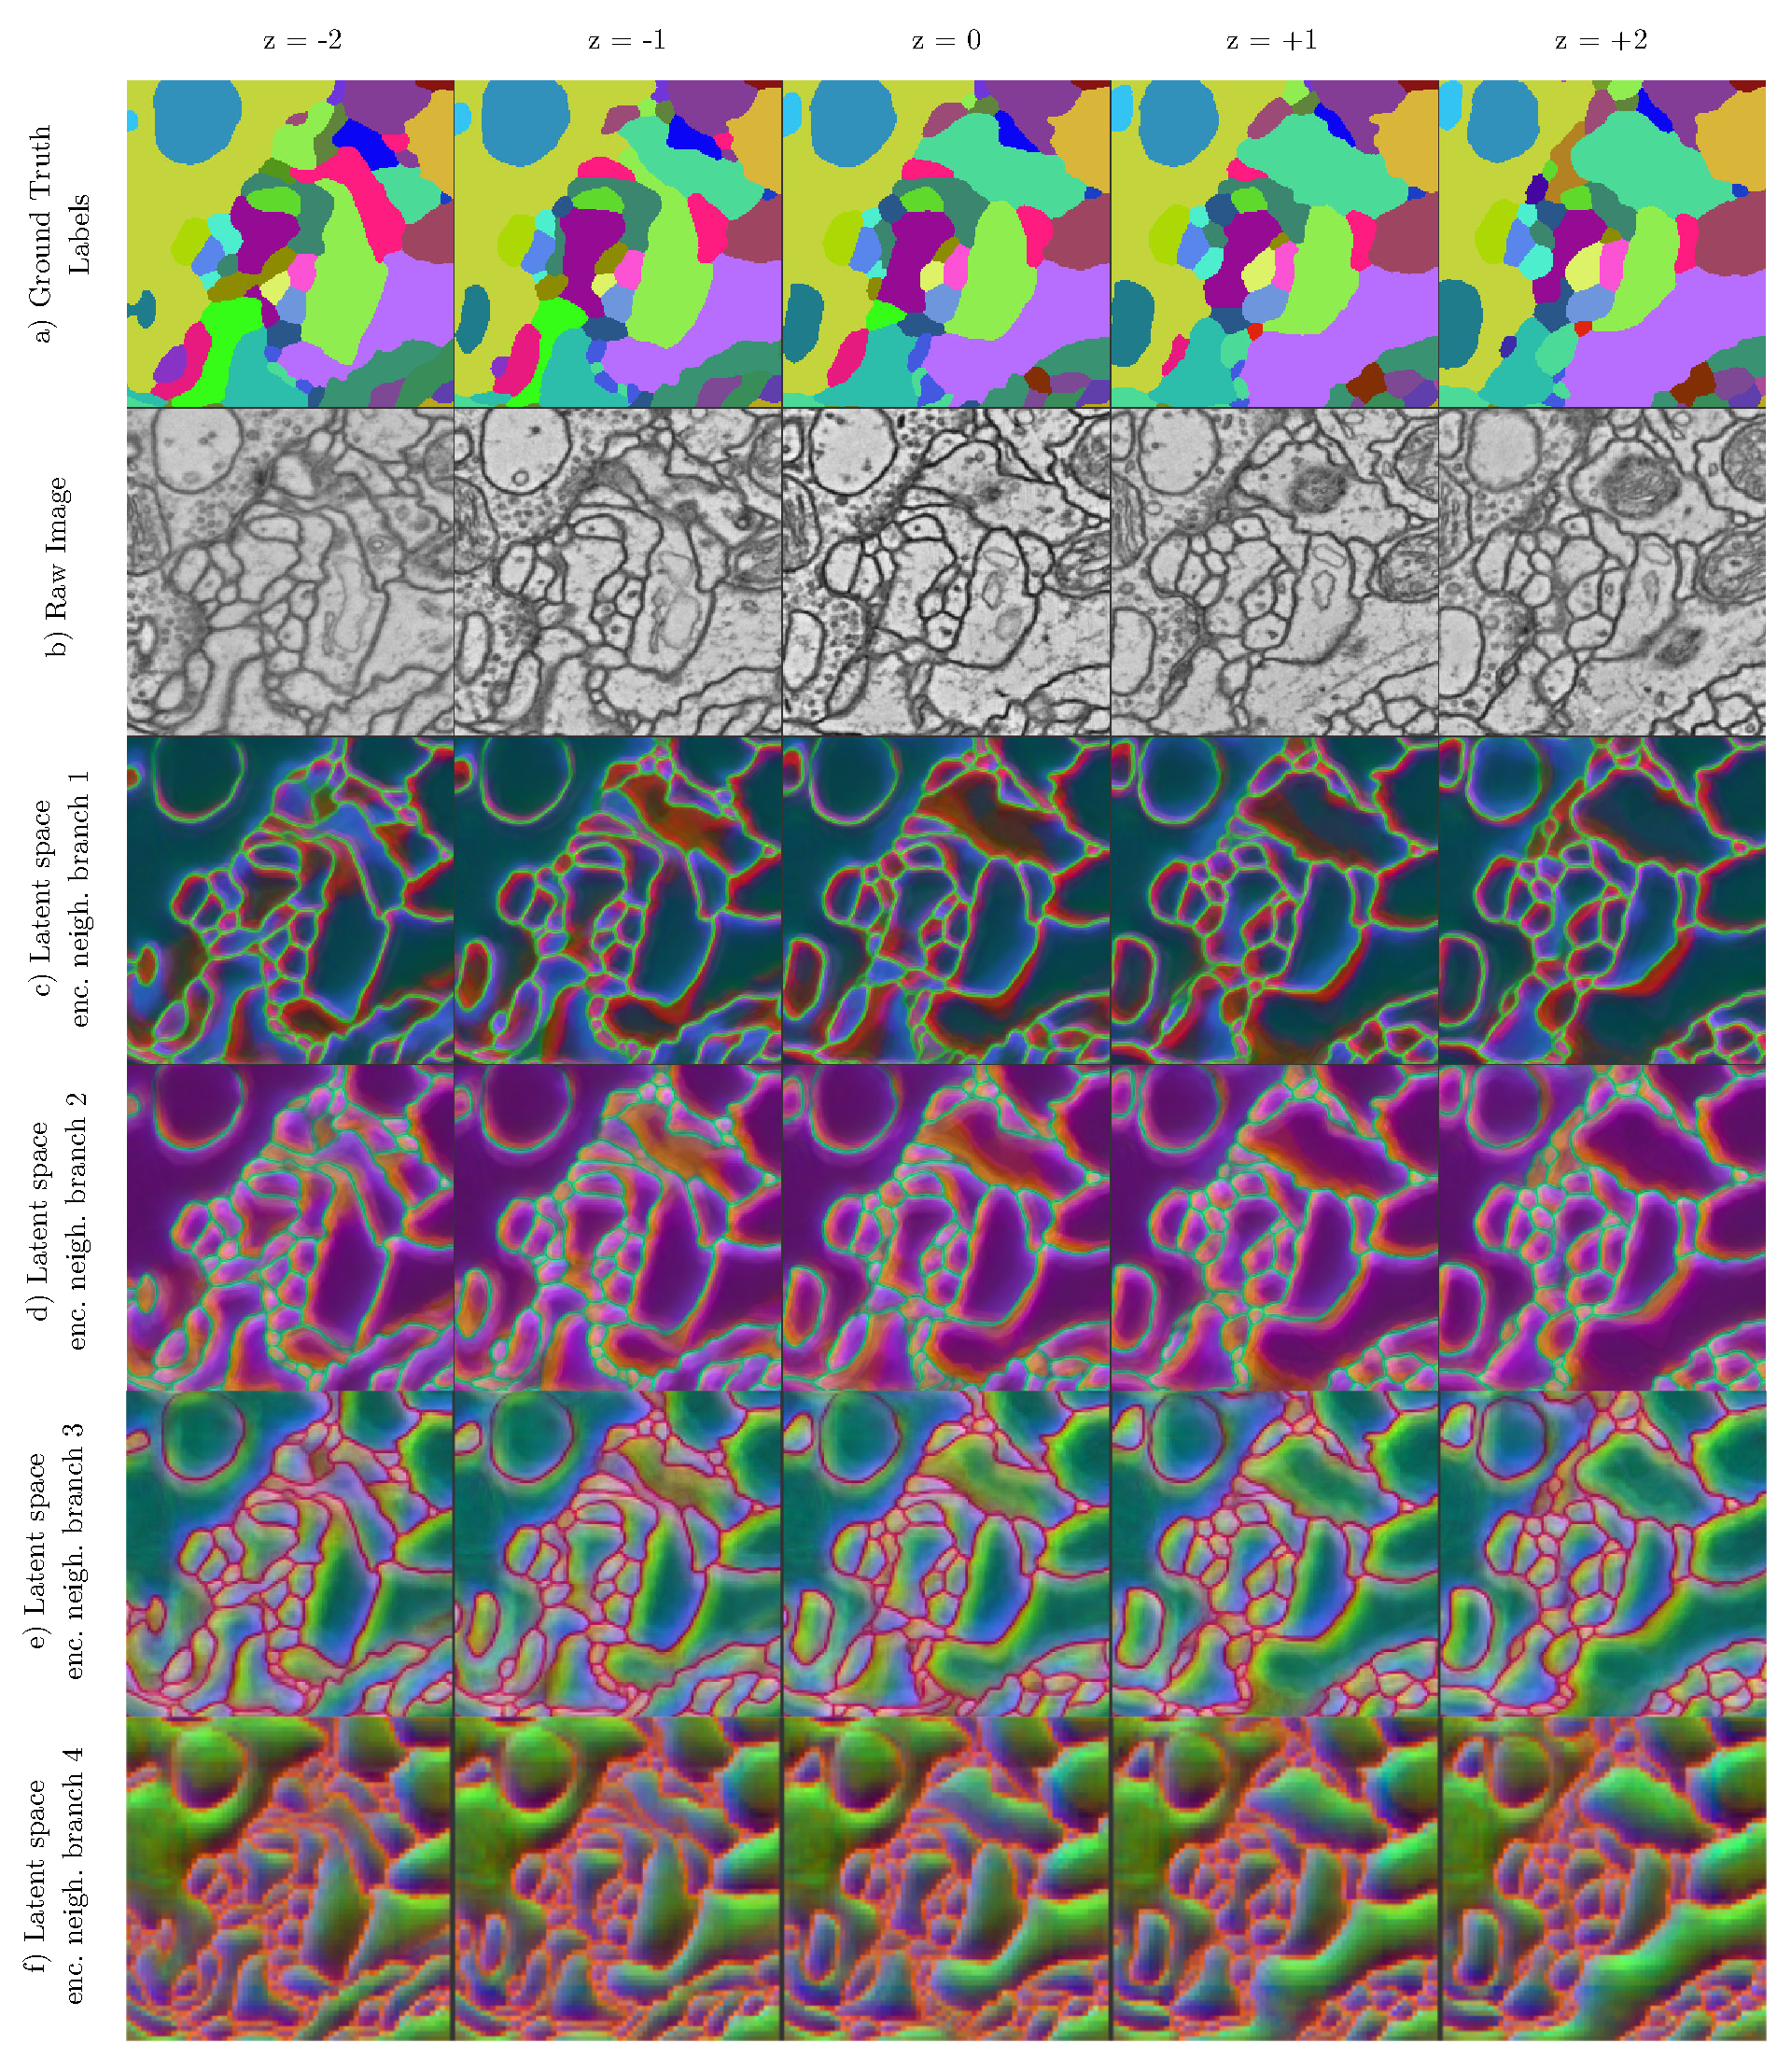
\includegraphics[width=\textwidth]{./figs/PCA_embeddings.pdf} % 0.45
        \vspace{1em}
        \caption{\textbf{Visualization of the predicted single-instance mask latent spaces} -- Each column represents a 2D image from the 3D stack (only five are shown here). \textbf{(a)} Ground-truth labels. \textbf{(b)} Raw image given as input to the model. \textbf{(c-d-e-f)} Visualization of the first three principal components of the $32$-dimensional mask latent spaces predicted by the \encBr branches ENB$_{i=1,2,3,4}$ in our model. Note how latent spaces learned at different levels of the U-Net pyramid show different feature-scales, because they encode \maskname masks at different resolutions.}
    \label{fig:PCA_embeddings}
\end{figure}

\begin{table}[t]
\small
\centering
  % {\renewcommand{\arraystretch}{1.3}
  % \resizebox{\textwidth}{!}{
        \begin{tabular}[t]{M{10em} M{8em} M{8em} M{8em} }
         % Method & \makecell{CREMI-Score \\(lower is better)} \\ \midrule 
\thead{Graph neighborhood\\structure\\(16 neighbors)} & \thead{SNB$_1$\\(18 neighbors)} &  \thead{SNB$_2$\\(10 neighbors)}  & \thead{SNB$_3$\\(10 neighbors)} \\ \toprule 
(0, 0, -1)      & (0, 0, -1)    & (0, 0, -1)    & (0, 0, -1) \\
(-1, 0, 0)      & (-1, 0, 0)    & (-4, 0, 0)    & (-4, 0, 0) \\
(0, -1, 0)     & (0, -1, 0)     & (0, -4, 0)    & (0, -4, 0) \\
(-4, 0, 0)     & (-4, 0, 0)     & (0, 0, -2)    & (0, 0, -2) \\
(0, -4, 0)     & (0, -4, 0)     & (0, 0, -3)    & (0, 0, -3) \\
(-4, -4, 0)    & (-4, -4, 0)    & (0, 0, -4)    & (0, 0, -4) \\
(4, -4, 0)     & (4, -4, 0)     & (-14, 0, 0)   & (-12, 0, 0) \\
(-4, 0, -1)     & (-4, 0, -1)   & (0, -14, 0)   & (0, -12, 0) \\
(0, -4, -1)     & (0, -4, -1)   & (-14, -14, 0) & (-12, -12, 0) \\
(-4, -4, -1)    & (-4, -4, -1)  & (14, -14, 0)  & (12, -12, 0) \\
(4, -4, -1)     & (4, -4, -1)   &  - & - \\
(0, 0, -2)      & (0, 0, -2)    & - & - \\
(-8, -8, 0)    & (0, 0, -3)     & - & - \\
(8, -8, 0)     & (0, 0, -4)     & - & - \\
(-12, 0, 0)    & (-8, -8, 0)    & - & - \\
(0, -12, 0)    & (8, -8, 0)     & - & - \\
-                & (-12, 0, 0)   & - & - \\
-               & (0, -12, 0)   & - & - \\
        \end{tabular}
        % }
        \vspace{3em}
        \caption{\textbf{Sparse neighborhood structures} --  
        In this table, we represent sparse neighborhood structures (see for example the one shown in Fig. \ref{fig:main_figure}a) as lists of offsets $(\delta_x,\delta_y, \delta_z)$ indicating the relative coordinates of neighboring pixels with respect to the central pixel.
        The first column shows the neighborhood structure of the pixel grid-graph, such that each pixel / node is connected to 16 neighbors. In the following columns, we provide the neighborhood structures predicted by the three \emph{\sparseBr branches} SNB$_i$ used in our model (see architecture in Fig. \ref{fig:model_architecture}).
        These neighborhood structures were inspired by the ones used in \cite{wolf2018mutex,lee2017superhuman} but were adapted to our version of the CREMI data that is downscaled by a factor $(\frac{1}{2},\frac{1}{2},1)$. Note that the offsets provided here are given in the downscaled resolution.} \label{tab:neighborhood_structures}
\end{table}



